\chapter{Data Preparation \& Model Training} \label{chap:training}

\section{Introduction}
The PU-Net and RNN layers provide a powerful way to learn the electronics response. Ideally, the ATN should be trained with paired waveforms of simulations and data. In reality, collecting such a paired dataset ranges from a major challenge to functionally impossible, depending on the desired population of events. Although we can simulate $\mathcal{T}_{Source}$ from an arbitrary $\mathcal{D}_{Source}$, obtaining a corresponding $\mathcal{T}_{Target}$ such that $\mathcal{D}_{Source} = \mathcal{D}_{Target}$ is difficult without precise knowledge of $P(X'|Y')$. Consequently, training must be performed on unpaired datasets, where $\mathcal{D}_{Source} \neq \mathcal{D}_{Target}$. The CycleGAN framework \cite{CycleGAN} provides an unsupervised learning approach to train the ATN using adversarial losses. We call this model, which combines all the features, the Cyclic Positional U-Net ({\cpunet}). {\cpunet} was initially developed by Aobo Li and has been refined and improved upon for this thesis. 

In this chapter, we describe the {\cpunet} training process. First, we outline the detector data collection and processing. Then, we discuss how we obtained the simulation dataset. Finally, we detail the training of the network using CycleGAN.

\section{Data selection}
The LEGEND Collaboration characterizes a subset of newly produced HPGe detectors at Oak Ridge National Laboratory (ORNL). We used characterization data from a LEGEND Inverted-Coaxial Point-Contact (ICPC) detector, V06643A, manufactured by ORTEC. These characterization measurements were made by Morgan Clark as part of her dissertation \cite{clark2023phdthesis}. The detector was mounted in a PopTop configuration, surrounded by lead shielding, and placed in a concrete alcove to reduce the external background. The data were taken with a flood Thorium-$232$ source placed on top of the detector. The detector signals were digitized using a FlashCam digitizer, and the \texttt{pygama} package \cite{pygama} was used to convert the FlashCam output to LEGEND HDF5 files.  The event energies were calibrated to convert the ADC units to keV. The energies were then corrected for charge trapping. Figure \ref{ch7_fig_eng_spec_comp} shows the final energy spectrum obtained from the detector.

The escape peaks in the spectrum are created from pair production events by a high-energy photon. In this process, the incident photon generates an electron-positron pair. The electron is collected by the detector, while the positron quickly annihilates, producing two additional gamma-ray photons. If all secondary gamma rays are fully absorbed within the detector, their combined energy yields a characterized peak in the energy spectrum, the Full Energy Peak (FEP).

If one of the annihilation gamma rays leaves the detector without depositing its energy, the spectrum shows a Single Escape Peak (SEP). This scenario results in a multi-site event because the signal comprises two distinct interactions within the detector: the collection of the pair-produced electron and the absorption of one of the two gamma rays. If both gamma rays escape the detector without interaction, a Double Escape Peak (DEP) is observed. This situation corresponds to a single-site event since the only interaction that contributes to the signal is the collection of the pair-produced electron. Tl-208 is part of the decay chain of $^{228}$Th and produces an FEP at $2614.53$ keV. Given that the mass of the electron is $511$ keV/c$^2$, the SEP peak occurs at $2103.53$ keV/c$^2$ and the DEP peak at $1592.53$ keV/c$^2$. 

The FEP peak is an excellent region for training, given that it has a lot of events and contains a mixture of single- and multi-site events. SEP and DEP peaks can then be used as a validation data set, evaluating the model's response to multi-site and single-site events, respectively.

\begin{figure}%[htb!]
  %[trim={left bottom right top},clip]
    \centering
    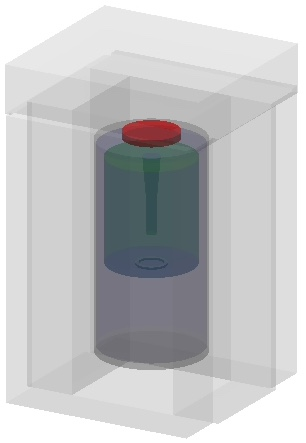
\includegraphics[width=0.4\linewidth]{ch7/figs/shielding.jpeg}
    \caption{The simulation geometry of the ORNL characterization setup, showing the detector in green, the source in red, the aluminum holder in dark grey, and the lead shielding in light grey.}
   \label{ch7_fig_g4simple_setup}
\end{figure}


\begin{figure}%[htb!]
\centering
  %[trim={left bottom right top},clip]
    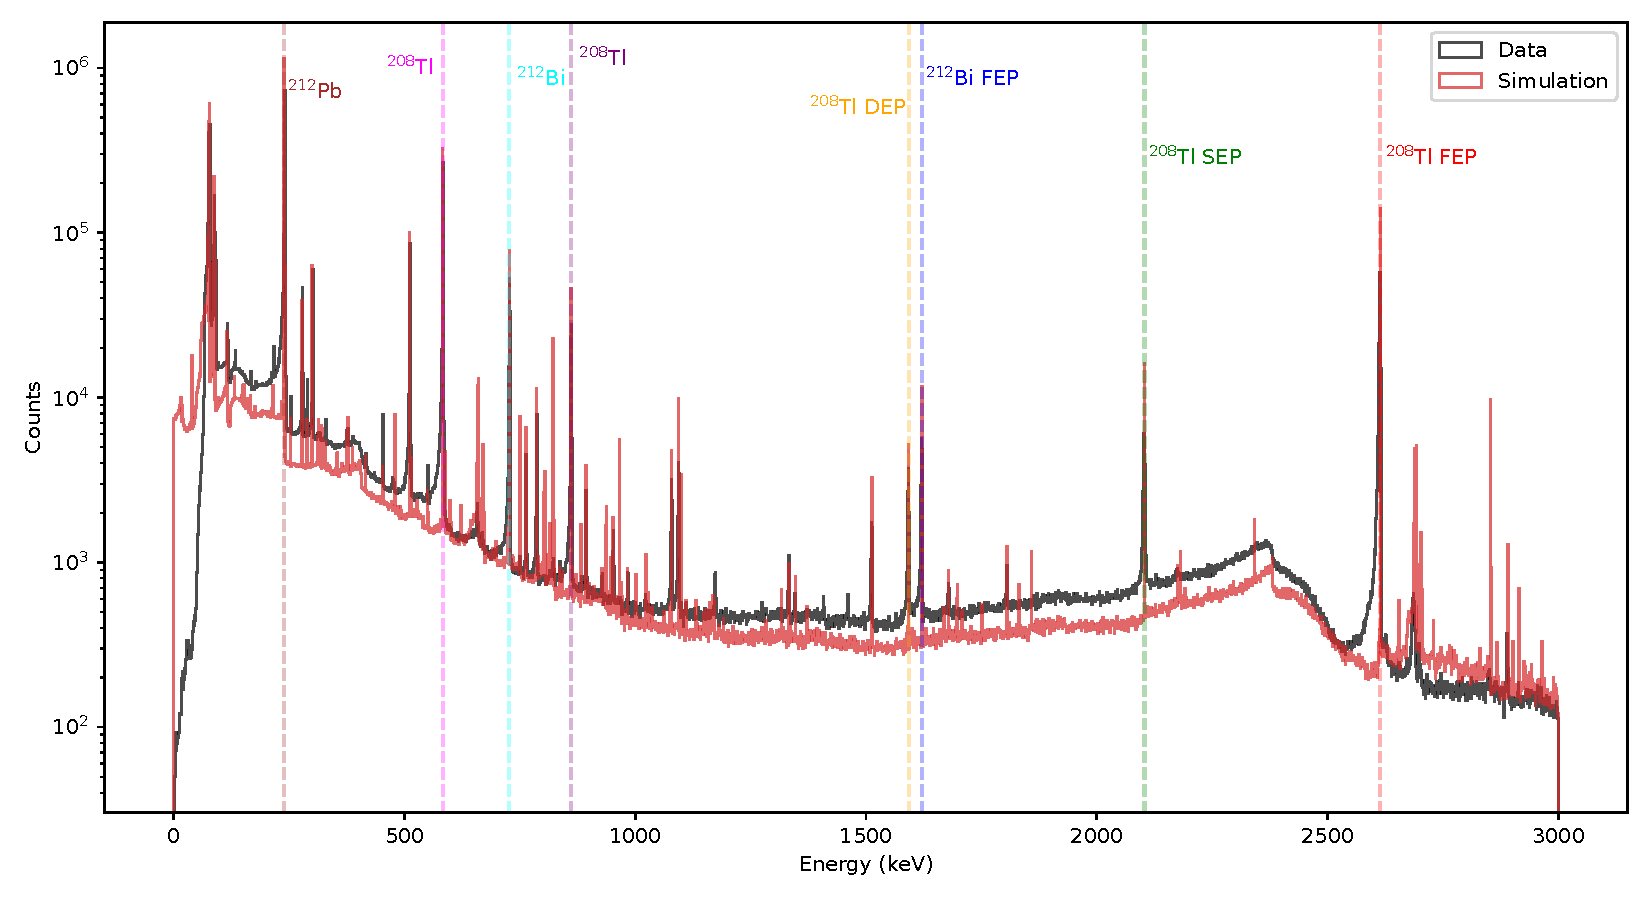
\includegraphics[width=0.99\linewidth,trim={0.5cm 0pc 0.5cm 0pc},clip]{ch7/figs/energy_spectrum_comparison.pdf}
    \caption{Calibrated energy spectrum from a $^{228}$Th source at ORNL compared to the Monte Carlo simulation results. Key peaks from $^{228}$Th source are labeled.}
   \label{ch7_fig_eng_spec_comp}
\end{figure}

\section{Simulations}
We designed a simple {\geant} setup geometry to simulate events in the ORNL characterization setup. The setup in {\geant} is shown in figure \ref{ch7_fig_g4simple_setup}. This includes a Germanium detector, a radioactive source, an Aluminum PopTop cryostat holder, surrounded by lead shielding. We simulated $100$ million $^{228}$Th decay events originating from the source and recorded their energy depositions within the germanium detector. Given the location of energy deposition within the detector, we used {\siggen} simulations to generate waveforms for hits in the DEP, SEP, and FEP energies. Figure \ref{ch7_fig_eng_spec_comp} also shows the simulated spectrum. The simulated energy spectrum was obtained by summing the energy depositions for a given event. The {\siggen} simulations used do not include any passivated surface effects. The {\siggen} simulations used treat every energy deposit as a single point charge and heuristically account for diffusion and self-repulsion by convolving the output signal with a $0.1$ mm FWHM Gaussian. We disabled the preamplifier integration by setting the shaping constant $\tau$ to zero.

Waveforms for multi-site events were created by energy-weighted summing of waveforms from individual hits. Figure \ref{ch7_fig_eng_dep_sim} shows the simulation process for a few events. The left panel depicts the hit locations of the particles for the events. Event $3$ and Event $4$ are effectively single-site, as the energy depositions occur very close to each other and thus produce single-site events. In Event $1$, the energy depositions result in two primary sites, giving rise to a two-site waveform. Event $2$ features a trace of energy deposition localized to three regions, which is classified as a three-site event. Events $3$ and $4$ have different drift times because they are deposited at different distances from the point contact.

\begin{figure}[htb!]
  %[trim={left bottom right top},clip]
    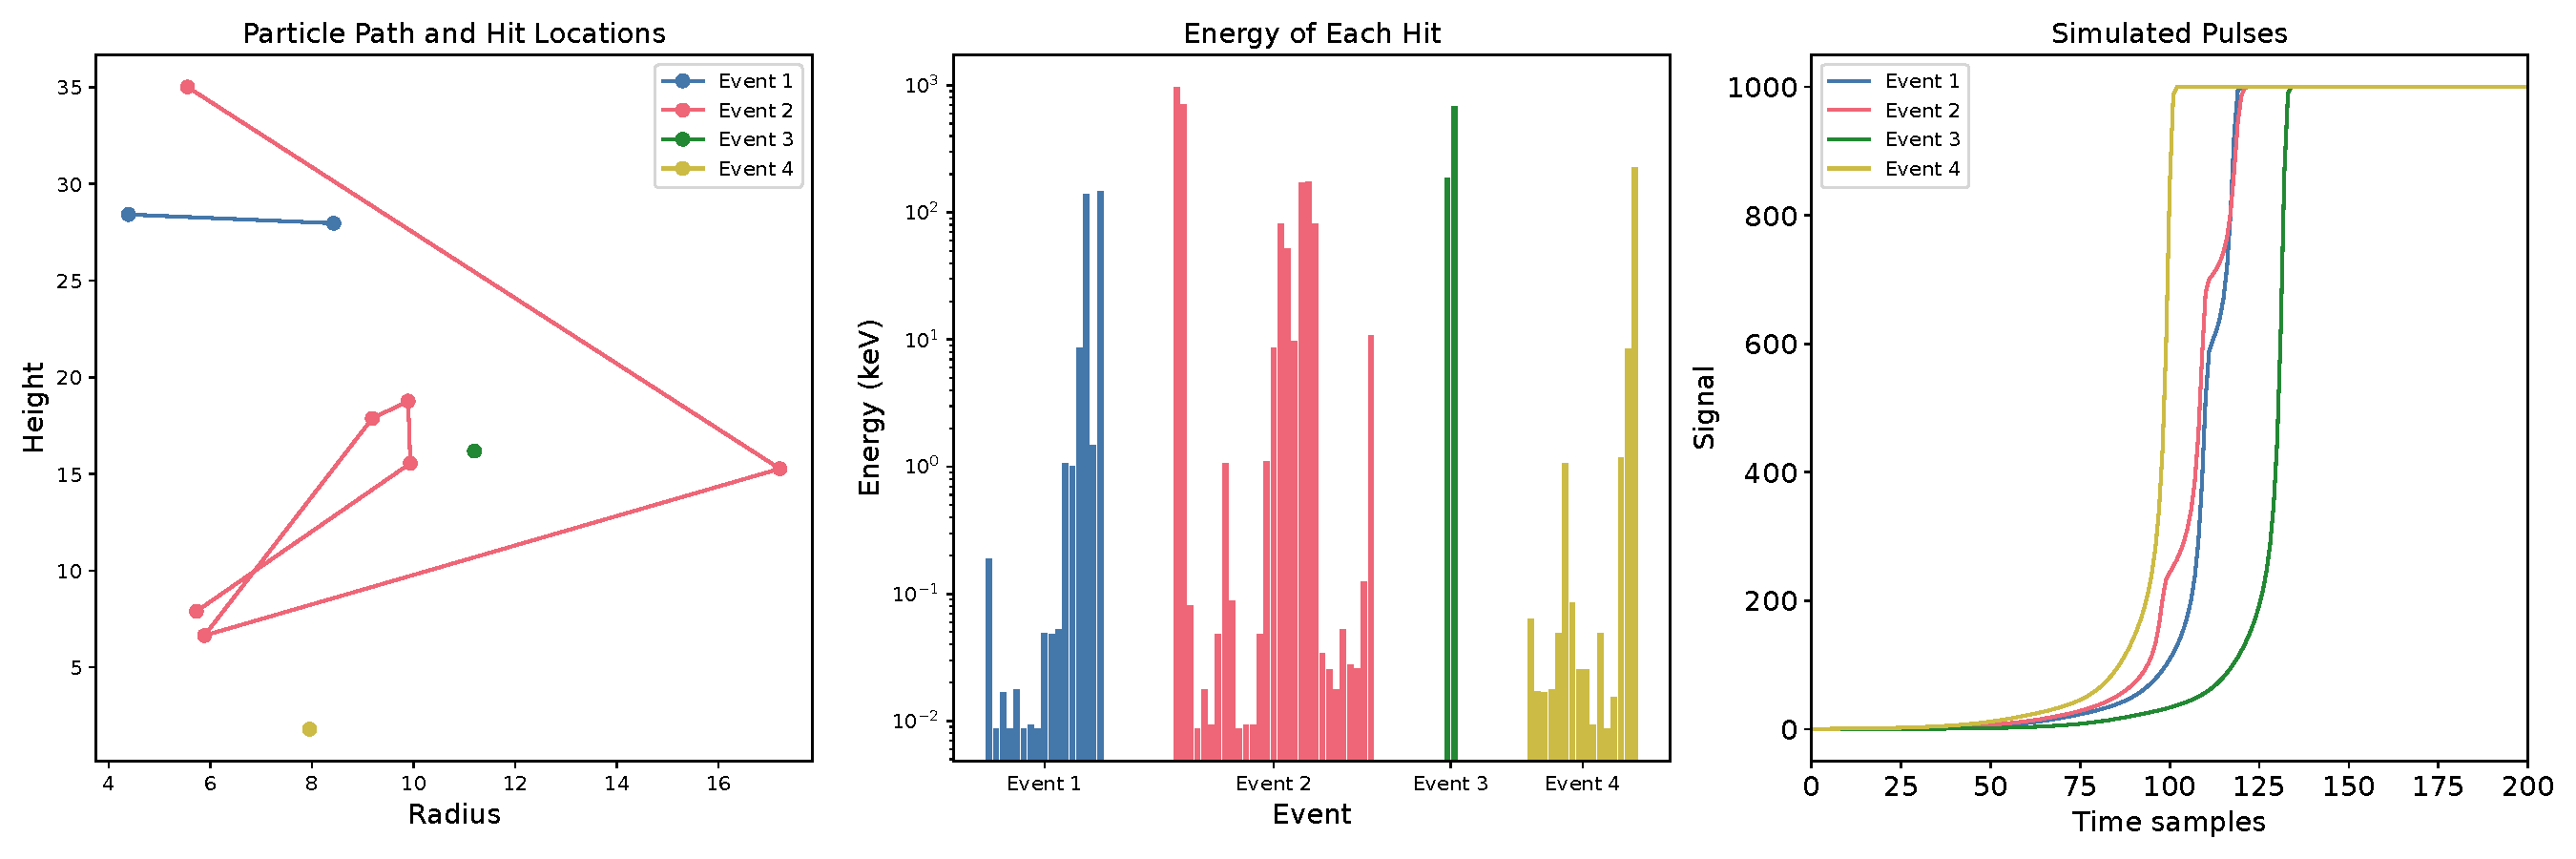
\includegraphics[width=0.99\linewidth,trim={1pc 0pc 1pc 0pc},clip]{ch7/figs/hit_sims.pdf}
    \caption{Production of energy weighted waveform in simulations for four events. Left figures show the location of hit locations for each event.  The magnitude of energy deposited for hits in each event is shown in middle figure. Right plot show the energy-weighted waveforms for the corresponding events. Hits produced using {\geant} simulations and waveforms are generated using {\siggen} software.}
   \label{ch7_fig_eng_dep_sim}
\end{figure}

\section{Post Processing}
Normalizing and aligning the waveforms is crucial for training the network. The simulated waveforms are already normalized between $0$ and $1$. The raw data waveforms are normalized by dividing by the $80\%$ of the average of the last five samples. Both waveforms are then vertically shifted so that the average of the first $200$ samples is zero. This ensures that all waveforms have their RC decay tails and baseline aligned, which can help the model learn the features better. Then we used the $99.9\%$ rise time to horizontally align the waveform. We found that this method was more effective for training the network than aligning by the zero time point, as the waveform shape at the end of the rise time is far more consistent between events than the shape corresponding to the beginning of the charge drift, which depends on the position of the energy deposition. The simulated waveforms are padded to ensure that there are $400$ samples on both sides of the $99.9\%$ rise time. The tail slope $\tau$ is calculated by the slope of a linear fit of the logarithm of the last $300$ waveform samples. Events with poor fit quality $\chi^2$ or anomalous tail slope $\tau$ are used to identify pile-up waveforms and remove them from training. Figure \ref{ch7_figs_in_out} shows the processed data and simulated waveforms that are fed into the neural networks.

\begin{figure}%[!htb]
    % \hspace{0.05\linewidth}
    %[trim={left bottom right top},clip]
    \centering
    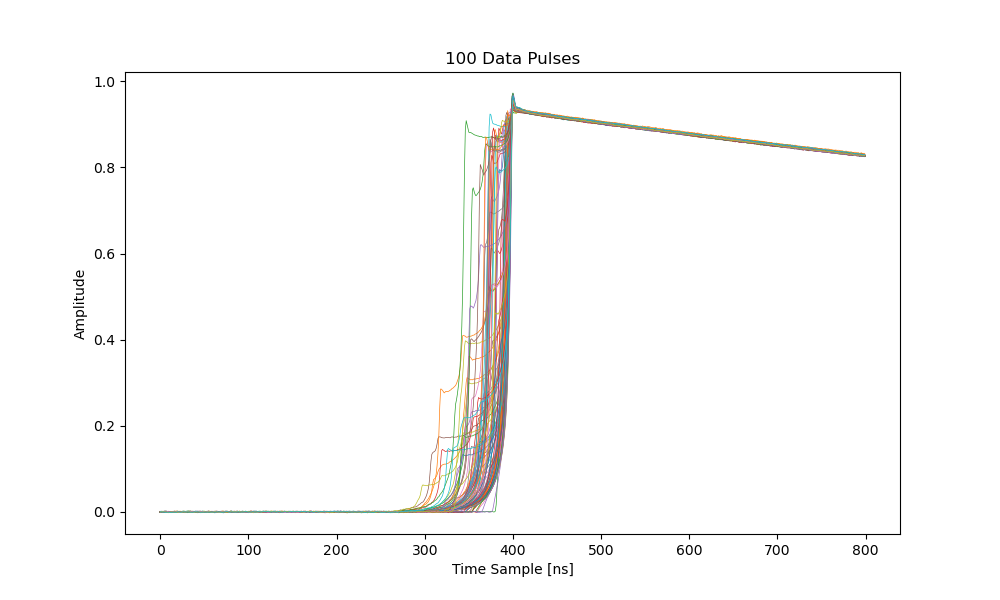
\includegraphics[width=0.9\linewidth,trim={4pc 0cm 6pc 1cm},clip]{ch7/figs/all_data_pulses.png}
    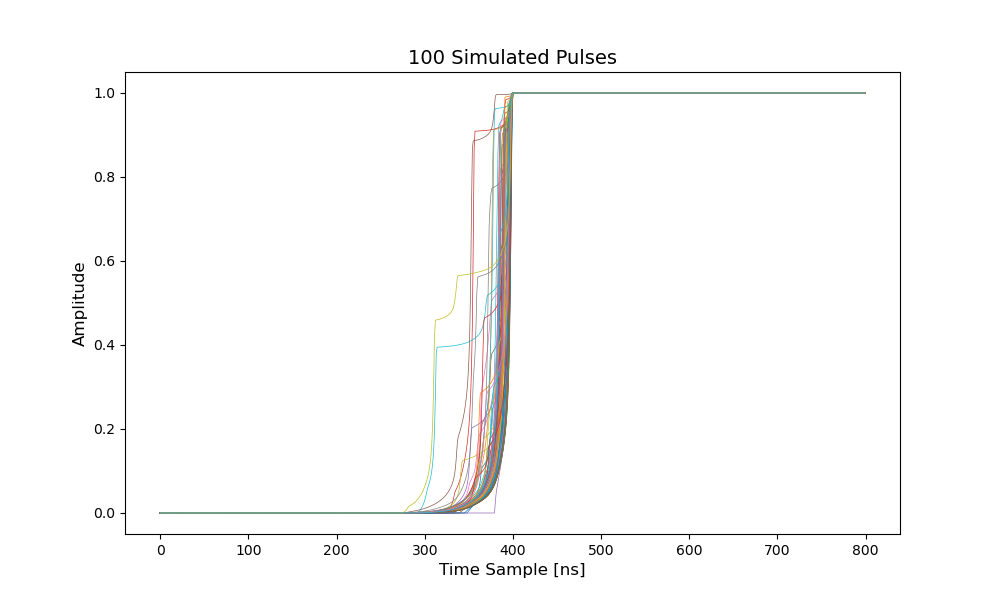
\includegraphics[width=0.9\linewidth,trim={4pc 0cm 6pc 1cm},clip]{ch7/figs/all_simulated_pulses.png}
    \caption{Input data and simulated waveforms. The waveforms are aligned by $99.9\%$ rise time. Data pulses are normalized by aligning the tail and baselines.}
   \label{ch7_figs_in_out}
\end{figure}

\section{Network Training}
The training and validation are performed in PyTorch \cite{pytorch}. We construct two networks: an ATN $\Lambda$ and an inverse ATN $\bar{\Lambda}$, both with the PU-Net structure. We then construct two RNN discriminator networks: a simulation discriminator $\delta_{S}$ and a data discriminator $\delta_{T}$ for the source and target waveforms, respectively. Figure \ref{fig:network_training} shows the overall training process.
\clearpage
\begin{figure}[htb!]
    \centering
    % \hspace{0.05\linewidth}
    %[trim={left bottom right top},clip]
    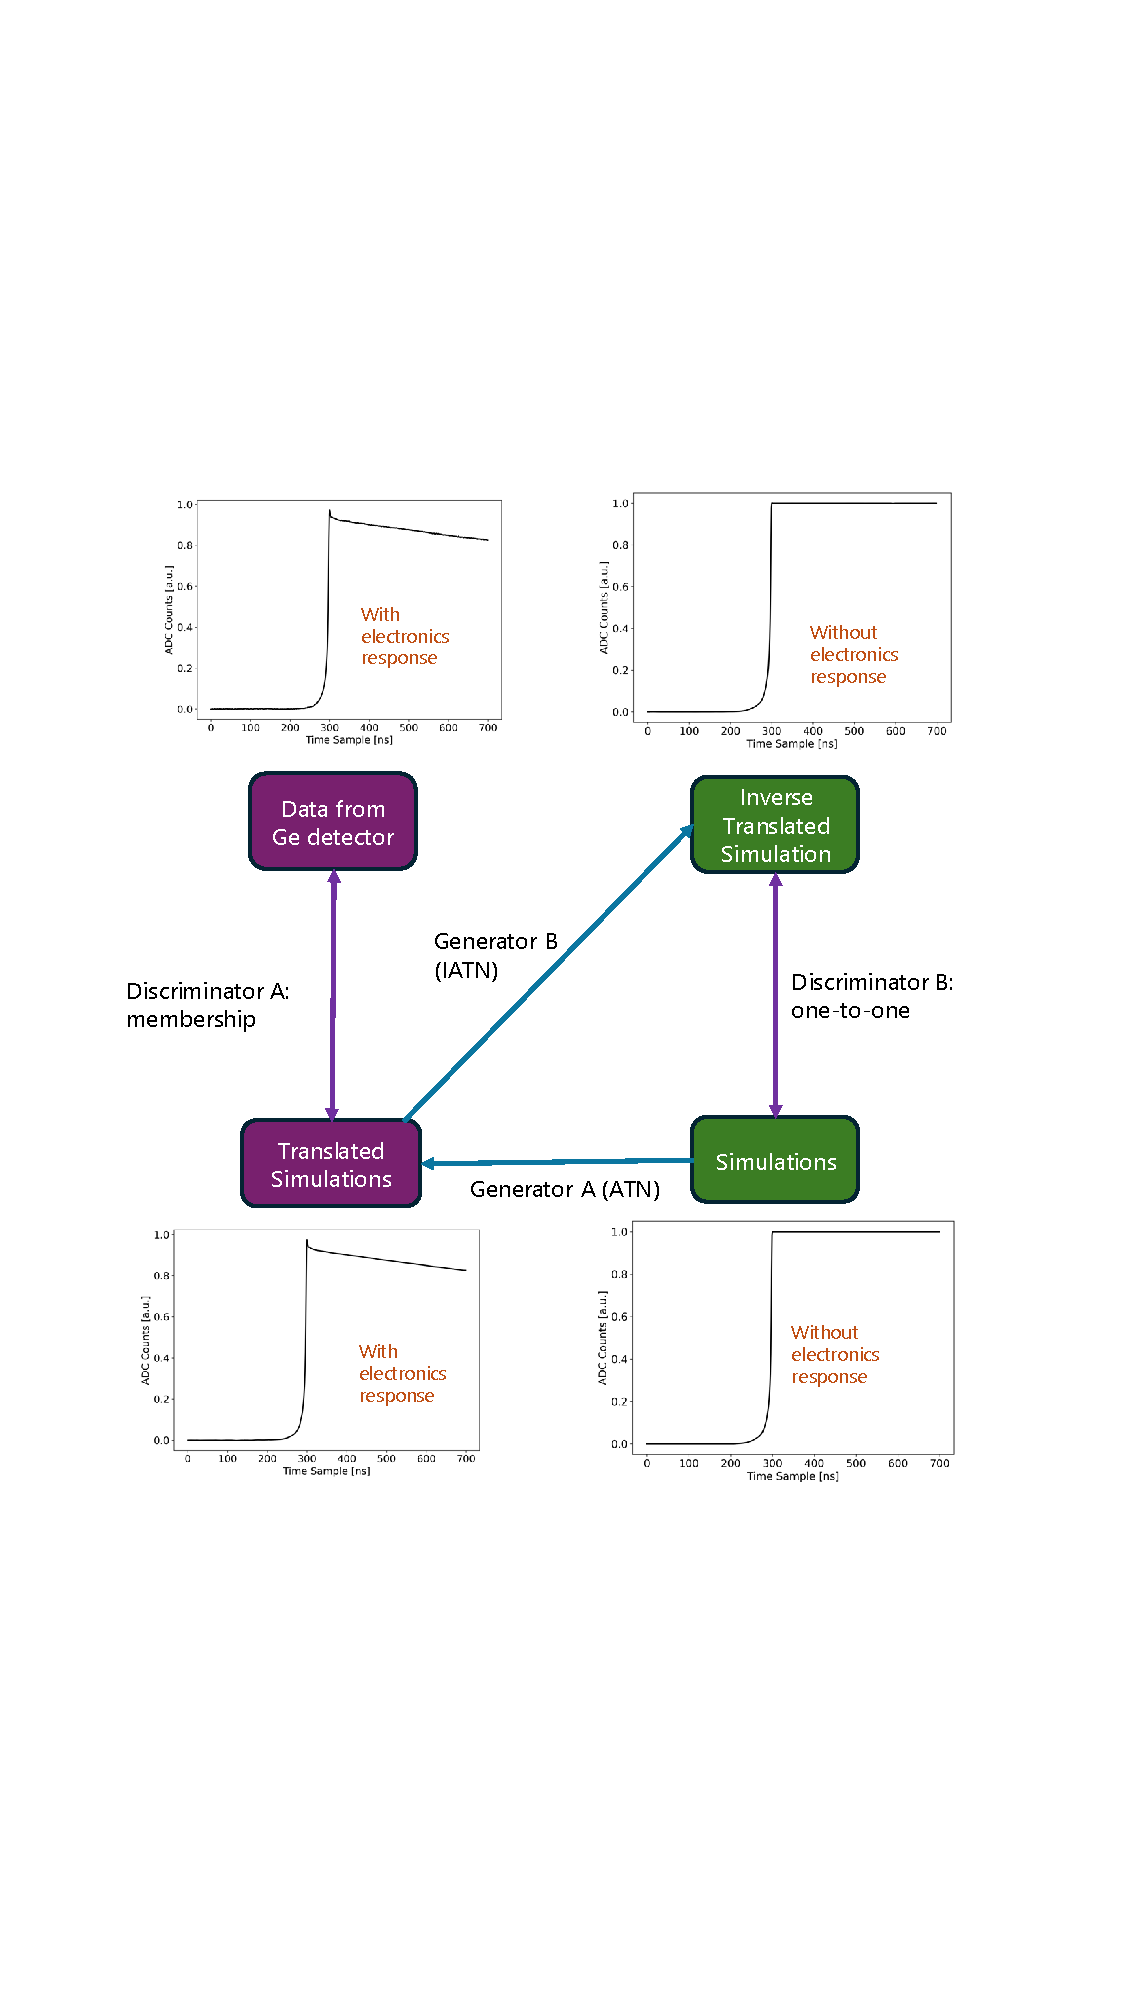
\includegraphics[width=0.99\linewidth,trim={5.5pc 20pc 6.3pc 19pc},clip]{ch7/figs/cycle_gan_training.pdf}
    \caption{Training in {\cpunet}. ATN transfers simulated waveforms to data-like waveforms, while the IATN transfers data waveforms to simulation-like waveforms. Discriminator A differentiates data-like waveforms outputs from the ATN from true data. Discriminator B differentiates simulation-like waveforms outputs from IATN from true simulations.}
   \label{fig:network_training}
\end{figure}

During training, a simulated waveform $X$ is first fed to $\Lambda$ to produce a translated waveform $\Lambda(X)$. The discriminator $\delta_{T}$ attempts to distinguish $\Lambda(X)$ from real data waveforms, while $\Lambda(X)$ attempts to `fool' $\delta_{T}$. Then $\Lambda(X)$ is fed to $\bar{\Lambda}$ to translate back to $\mathcal{X}$ space by $\bar{\Lambda}(\Lambda(\mathcal{X}))$. A second discriminator $\delta_{S}$ attempts to distinguish $\bar{\Lambda}(\Lambda(\mathcal{X}))$ from $\mathcal{X}$, while $\bar{\Lambda}$ attempts to `fool' $\delta_{S}$. The $\mathcal{X}\rightarrow{}\Lambda(\mathcal{X})\rightarrow{}\bar{\Lambda}(\Lambda(\mathcal{X}))$ translation path is termed the forward cycle. The same process is performed in the other direction, starting with the detector waveform $\mathcal{X}'\rightarrow{}\bar{\Lambda}(\mathcal{X}')\rightarrow{}\Lambda(\bar{\Lambda}(\mathcal{X}'))$ and called the backward cycle.

\section{Loss Functions}
Since we do not have a labeled training sample of matched data and simulation waveforms, we cannot use a direct comparison loss. Instead, we define three losses that are optimized during training to help the network learn the translations. $L_{\mathrm{Identity}}$ ensures that the identity relationship such that when a real detector waveform $X'$ is fed into $\Lambda$, whose goal is to produce a detector-like waveform, the waveform should not be modified by $\Lambda$. This is shown in the equation \ref{eq:loss_ided}. 

\begin{equation}\label{eq:loss_ided}
    L_{\mathrm{Identity}} = |X' - \Lambda(X')|
\end{equation}

The cycle-consistent loss in equation \ref{eq:loss_cyc} ensures that the circular translation path preserves the original waveform shape. The forward cycle is when the waveform is fed into ATN to produce a detector-like waveform, which is then passed through IATN to produce a simulation-like waveform. This should return the original simulated waveform, and the cycle loss calculates the loss associated with this whole cycle. Similarly, the backward cycle loss is when data is passed through IATN to get a simulation-like waveform, which is passed through ATN to get the original data waveform back. The cycle-consistent loss acts in place of a direct comparison loss to ensure that the underlying physical features that are encoded in a waveform (e.g. multi-site vs. single-site, or energy deposition location) are not destroyed by the translation networks.

\begin{equation}\label{eq:loss_cyc}
    L_{\mathrm{Cycle}} = |X - \bar{\Lambda}(\Lambda(X))|
\end{equation}

In both cycles and identities, the waveform is compared with another waveform. For such a comparison, we define a specialized mean absolute error (L1 loss) that emphasizes different parts of the waveform by assigning them varying weights. It is designed to give more importance to the rising and falling edges of the waveform, which are critical for accurate pulse shape analysis.

The adversarial loss calculates the loss associated with the generator and discriminator `fooling' each other. The discriminator takes in the waveform from the generator and outputs a single value between 0 and 1. A value close to 1 means that the discriminator classifies it as real data, while a value close to zero means that the discriminator classifies it as simulated waveform. 

Suppose we start with a simulated waveform $X$, and let $X' = \Lambda(X)$ be the output of the generator $\Lambda$. The adversarial loss for the generator is equal to $\delta_T(X')$, so that it is encouraged to produce a waveform that the discriminator classifies as data. The discriminator loss for $\delta_T$ is computed as $1 - \delta_T(X')$, encouraging it to classify it as simulation. Both losses are quantified using the binary cross-entropy loss, as shown in equation \ref{ch7_eq_loss_gan}:

\begin{equation}\label{ch7_eq_loss_gan}
    L_{\mathrm{Adversarial}} = E_{\mathcal{X'}}\log(\delta(X')) - E_{\Lambda(\mathcal{X})}\log(1 - \delta(\Lambda(X)))
\end{equation}

An additional three complementary losses are defined for the detector waveform translation path. Therefore, a total of eight losses are optimized during training: six are associated with the generators and two are associated with the discriminators. The loss calculations are summarized in table \ref{ch7_tab_loss_summary}.

\begin{table}%[ht!]
\centering
\renewcommand{\arraystretch}{1.5} % Adjust row height for readability
\setlength{\tabcolsep}{2.0pt} % Adjust column spacing
\begin{tabular}{|p{0.18\linewidth}|p{0.39\linewidth}|p{0.22\linewidth}|p{0.15\linewidth}|}
\hline
Loss                & Calculation                             & Type of Loss                                  & Optimizer   \\ \hline
Identity Losses    & Data - ATN(Data)                                & \multirow{3}{=}{Custom L1 Loss} & \multirow{8}{=}{Optimizer 1} \\
                             & Sim - IATN(Data)                                 &                                                       &                       \\ \cline{1-3}
Cycle Losses        & Data – ATN(IATN(Data))                         & \multirow{3}{=}{Custom L1 Loss} &                       \\
                             & Sim – IATN(ATN(Sim))                          &                                                       &                       \\ \cline{1-3}
Generator Losses    & Disc B (IATN(Data))                              & \multirow{2}{=}{Binary Cross Entropy}                &                       \\
                             & Disc A (ATN(Sim))                              &                                                       &                       \\ \hline
Discriminator A     & {[Disc A(Data) - 1]} + {[Disc A(Sim) - 0]}        &  Binary Cross Entropy                                & Optimizers 2 \\ \hline
 Discriminator B    & {[Disc B(Sim) - 1]} + {[Disc B(Data) - 0]}        &   Binary Cross Entropy                                &   Optimizers 3             \\ \hline
\end{tabular}
\caption{Overview of Loss Calculations, Loss Types, and Optimizers.}
\label{ch8_tab_loss_summary}
\end{table}


AdamW \cite{adam_w_paper} optimizers are used for all losses. Compared to the traditional Adam optimizer, AdamW applies weight decay as a separate step during gradient descent optimization. This avoids interference with the learning rate schedule and helps stabilize the training process. In total, we define three optimizers, as shown in table \ref{ch7_tab_loss_summary}. The six losses for ATN and IATN are optimized together, and the discriminators each have their own optimizers.

\section{Hyperparameter Tuning}
Achieving stability in CycleGAN training can be challenging. This is because the loss optimization process is complex as there is not one metric such as mean squared difference being optimized. Training must balance the learning progress of generators and discriminators while preventing gradients from exploding or imploding to zero. To improve training, we introduced hyperparameters at different levels of the model that are summarized in table \ref{tab:hyperparameters}.

\begin{table}%[htb!]
\centering
\renewcommand{\arraystretch}{1.5} % Adjust row height for readability
\setlength{\tabcolsep}{2pt} % Adjust column spacing
\begin{tabular}{|p{0.18\linewidth}|p{0.12\linewidth}|p{0.65\linewidth}|}
\hline
\textbf{Hyperparameter}       & \textbf{Value} & \textbf{Description} \\ \hline
batch\_size          & 32             & Number of pulses used in one training iteration. \\ \hline
baseline\_len        & 200            & Number of samples assigned to baseline portion of the waveform. \\ \hline
rising\_edge\_len    & 250            & Number of samples assigned to the rising edge of the waveform. \\ \hline
tail\_len            & 350            & Number of samples assigned to the RC decay tail of the waveform. \\ \hline
baseline\_weight     & 3.0            & Weight given to baseline portion of the waveform in the loss. \\ \hline
ris\_edge\_weight    & 10.0           & Weight given to rising edge portion of the waveform in the loss. \\ \hline
tail\_weight         & 7.0            & Weight given to RC decay tail portion of the waveform in the loss. \\ \hline
iters                & 7000           & Maximum number of iterations for training. \\ \hline
decay                & 1000           & Iteration at which learning rate starts to decay. \\ \hline
lrate\_gen           & $1 \times 10^{-3}$ & Learning rate for the generator networks. \\ \hline
lrate\_disc          & $1 \times 10^{-3}$ & Learning rate for the discriminator networks. \\ \hline
cyc\_loss\_weight    & 20             & Weight of the cycle consistency losses.  \\ \hline
iden\_loss\_weight   & 5              & Weight of the identity loss. \\ \hline
gan\_loss\_weight    & 9              & Weight of the generator loss. \\ \hline
max\_grad\_norm      & 100            & Maximum gradient norm for gradient clipping. \\ \hline
w\_decay             & $1 \times 10^{-4}$ & Weight decay in the optimizers. \\ \hline
n\_disc\_iters       & 30             & Number of iterations after which the discriminators are updated. \\ \hline
\end{tabular}
\caption{Hyperparameters used for CPU-Net training.}
\label{tab:hyperparameters}
\end{table}


It was found that the discriminator typically overpowers the generator, since the generator has a more complex task of generating waveforms while maintaining cycle and identity consistency and also fooling the discriminator. To balance this, we update the weights of the generators more frequently than the discriminators. We introduced a hyperparameter for the number of intervals after which the discriminator is updated. This allowed the generator enough steps to adapt to changes in the discriminator without destabilizing the adversarial process.

The weighting of the adversarial, cycle-consistency, and identity losses enables fine-tuning the learning of the generators. At some point, the generator will have learned just enough to fool the discriminator, and further learning might be hampered. The loss weights are used to optimize the generator to learn translation, such as the cycle and identity consistency even if it has been successful in overpowering the discriminator. These hyperparameters are carefully tuned to achieve a balance, as values that are too high will cause the gradient to explode; too low will cause the model not to learn much. 

We also introduced a learning rate decay for the optimizers. In the beginning, the learning rate is intentionally kept high for the model to explore the entire parameter space. Then, the learning rate decays linearly to help it converge in the right direction. This is particularly important for the ATN optimizer, as it is optimizing six losses, and this ensures that all the space is explored.

To prevent overfitting during training, weight decay is applied to the optimizers so that it penalizes large weights and ensures generalization among all parameters. Gradient clipping is applied, limiting the norm of gradients during training and preventing exploding gradients, particularly in the layers of the U-Net. The threshold for clipping the magnitude of gradients is kept high since the loss is multiplied by different loss weights multiple times, which can increase the magnitude.

Together, these parameters enable precise fine-tuning {\cpunet} training to obtain the right balance during training. A single training takes about 1 GPU hour on an NVIDIA A100 GPU. The trained {\cpunet} generates both an ATN and an inverse ATN, enabling bidirectional translation between the simulation and data domains. The ATN is the primary focus of this work, but the reverse ATN can also enhance analysis by refining the waveform reconstruction. In the next chapter, we discuss some results from the ATN output.